\documentclass[10pt, twocolumn]{article}
\usepackage[margin=0.75in]{geometry}
\usepackage{graphicx}
\usepackage{tikz}
\usepackage{pgfplots}
\usepackage{booktabs}
\usepackage{amsmath}
\usepackage{amssymb}
\usepackage{hyperref}
\usepackage{xcolor}
\usepackage{caption}
\usepackage{subcaption}
\usepackage{fancyhdr}
\usepackage{enumitem}
\usepackage{listings}
\usepackage{microtype}
\usepackage{tabularx}
\usepackage{multirow}

\pgfplotsset{compat=1.18}
\usetikzlibrary{arrows.meta, positioning, shapes.geometric, fit, calc, backgrounds}

% ORCID icon (inline TikZ)
\definecolor{orcidgreen}{HTML}{A6CE39}
\newcommand{\orcidicon}{%
  
\begin{tikzpicture}[baseline=(char.base)]
    \node[circle, fill=orcidgreen, inner sep=0pt, minimum size=2.2ex] (char)
      {\textcolor{white}{\sffamily\bfseries\scriptsize iD}};
  \end{tikzpicture}%
}

% Color palette (matches sister papers)
\definecolor{amblue}{HTML}{2563EB}
\definecolor{amdarkblue}{HTML}{1E40AF}
\definecolor{amteal}{HTML}{0D9488}
\definecolor{amorange}{HTML}{EA580C}
\definecolor{amgray}{HTML}{6B7280}
\definecolor{amlightgray}{HTML}{F3F4F6}
\definecolor{amgreen}{HTML}{059669}
\definecolor{amred}{HTML}{DC2626}
\definecolor{ampurple}{HTML}{7C3AED}

\lstset{
  basicstyle=\ttfamily\scriptsize,
  keywordstyle=\color{amblue}\bfseries,
  commentstyle=\color{amgray}\itshape,
  stringstyle=\color{amteal},
  breaklines=true,
  frame=single,
  rulecolor=\color{amgray!30},
  backgroundcolor=\color{amlightgray},
  numbers=left,
  numberstyle=\tiny\color{amgray},
  tabsize=2
}

\hypersetup{
  colorlinks=true,
  linkcolor=amblue,
  citecolor=amblue,
  urlcolor=amblue,
}

\pagestyle{fancy}
\fancyhf{}
\renewcommand{\headrulewidth}{0.4pt}
\fancyhead[L]{\small\textit{AgenticCognition: Longitudinal User Modeling}}
\fancyhead[R]{\small\thepage}

\title{\textbf{AgenticCognition: A Living Model Architecture for\\Longitudinal User Modeling in AI Agents}}
\author{Omoshola Owolabi\,\orcidicon \\
  \small Researcher -- AI/ML \\
  \small Agentra Labs \\
  \small \texttt{omoshola.owolabi@agentralabs.tech}}
\date{March 2, 2026}

\begin{document}
\maketitle
\thispagestyle{fancy}

% ============================================================================
% ABSTRACT
% ============================================================================
\begin{abstract}
AI agents operate without persistent understanding of the humans they serve. Each conversation begins from zero---no knowledge of the user's beliefs, values, decision patterns, or psychological landscape. Current approaches to user modeling treat the person as a static profile: a list of preferences to be looked up. We present AgenticCognition, a system that models users as \emph{living entities} with belief physics, shadow psychology, decision fingerprints, and drift tracking. Beliefs are not inert records but physical objects that crystallize over time, entangle with other beliefs, exert gravitational pull, and collapse under contradiction. The system detects shadow beliefs the user holds but would deny, projects blind spots in self-assessment, and tracks how values shift across interactions. We implement AgenticCognition in 12{,}099 lines of Rust across 4 crates (core library, MCP server, CLI, and FFI bindings), validated by 229 tests with zero failures. Criterion benchmarks on Apple M4 Pro demonstrate sub-microsecond query performance: \texttt{get\_belief\_graph} in 2.0\,$\mu$s, \texttt{soul\_reflection} in 1.5\,$\mu$s, \texttt{predict\_preference} in 2.5\,$\mu$s, and model persistence at 5.2\,ms save / 88\,$\mu$s load for 100-belief models. The system exposes 14 MCP tools, 5 resources, and 4 prompt templates, enabling any MCP-compatible AI agent to develop genuine, evolving understanding of the humans it works with. AgenticCognition is Sister \#9 of 25 in the Agentra ecosystem.
\end{abstract}

% ============================================================================
% 1. INTRODUCTION
% ============================================================================
\section{Introduction}
\label{sec:intro}

The transformer architecture~\cite{vaswani2017attention} has produced language models capable of nuanced conversation, complex reasoning, and creative generation. Yet these models understand \emph{nothing} about the person they are speaking with. Every conversation begins with the same blank slate. An agent that has helped a user make hundreds of decisions cannot recall a single preference, predict a single choice, or detect a single blind spot. The user is a stranger every time.

Current approaches to this problem fall into two categories, both inadequate. \emph{Static profiles}~\cite{brusilovsky2001adaptive} store explicit preferences (``prefers dark mode,'' ``uses Python'') as key-value pairs, treating the user as a configuration file. \emph{Conversation histories}~\cite{packer2023memgpt} preserve raw dialogue, relying on retrieval-augmented generation to surface relevant context. Neither captures the dynamic, interconnected, often contradictory nature of human cognition.

The core insight of this work is that a user is not a profile but a \emph{living system}. People do not have preferences---they have beliefs that crystallize over time, values that drift under pressure, shadow aspects they cannot see, and decision patterns that reveal more than their words. Modeling a user requires modeling these dynamics: the physics of belief formation, the topology of self-concept, the archaeology of value change.

We present AgenticCognition, a Rust library and MCP server that implements this vision. The system introduces six novel modeling subsystems: (1)~a \emph{living user model} with vitals, consciousness state, and lifecycle events; (2)~\emph{belief physics} where beliefs crystallize, entangle, exert gravity, and collapse; (3)~\emph{self-concept topology} mapping psychological peaks, valleys, and blind canyons; (4)~\emph{shadow psychology} detecting denied beliefs, projections, and blind spots; (5)~\emph{decision fingerprinting} across eight trait axes; and (6)~\emph{drift tracking} monitoring how values shift over time.

The remainder of this paper is organized as follows. Section~\ref{sec:related} surveys existing approaches to user modeling and cognitive architectures. Section~\ref{sec:architecture} presents the six subsystems in detail. Section~\ref{sec:evaluation} reports benchmark results from Criterion. Section~\ref{sec:mcp} describes the MCP integration and test validation. Section~\ref{sec:discussion} discusses implications and limitations. Section~\ref{sec:conclusion} concludes.

% Figure 1: Motivating comparison
\begin{figure*}[t]
\centering
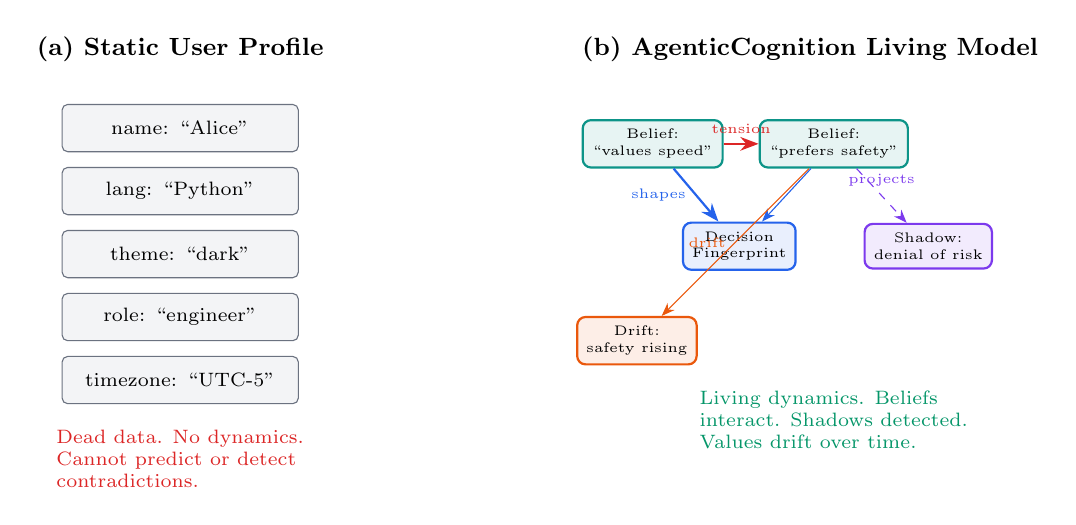
\begin{tikzpicture}[
  every node/.style={font=\small},
  staticbox/.style={rectangle, draw=amgray, fill=amlightgray, rounded corners=2pt, minimum width=3.0cm, minimum height=0.6cm, align=center, font=\scriptsize},
  livingnode/.style={rectangle, rounded corners=3pt, draw=amblue, fill=amblue!10, minimum width=1.3cm, minimum height=0.5cm, font=\tiny, align=center, thick},
  beliefnode/.style={rectangle, rounded corners=3pt, draw=amteal, fill=amteal!10, minimum width=1.3cm, minimum height=0.5cm, font=\tiny, align=center, thick},
  shadownode/.style={rectangle, rounded corners=3pt, draw=ampurple, fill=ampurple!10, minimum width=1.3cm, minimum height=0.5cm, font=\tiny, align=center, thick},
  driftnode/.style={rectangle, rounded corners=3pt, draw=amorange, fill=amorange!10, minimum width=1.3cm, minimum height=0.5cm, font=\tiny, align=center, thick},
]

% Left side: Static Profile
\node[font=\small\bfseries] at (-4.5, 3.2) {(a) Static User Profile};
\node[staticbox] (s1) at (-4.5, 2.2) {name: ``Alice''};
\node[staticbox] (s2) at (-4.5, 1.4) {lang: ``Python''};
\node[staticbox] (s3) at (-4.5, 0.6) {theme: ``dark''};
\node[staticbox] (s4) at (-4.5, -0.2) {role: ``engineer''};
\node[staticbox] (s5) at (-4.5, -1.0) {timezone: ``UTC-5''};

\node[font=\scriptsize\color{amred}, align=left] at (-4.5, -2.0) {Dead data. No dynamics.\\Cannot predict or detect\\contradictions.};

% Right side: Living Model
\node[font=\small\bfseries] at (3.5, 3.2) {(b) AgenticCognition Living Model};

\node[beliefnode] (b1) at (1.5, 2.0) {Belief:\\``values speed''};
\node[beliefnode] (b2) at (3.8, 2.0) {Belief:\\``prefers safety''};
\node[livingnode] (d1) at (2.6, 0.7) {Decision\\Fingerprint};
\node[shadownode] (sh1) at (5.0, 0.7) {Shadow:\\denial of risk};
\node[driftnode] (dr1) at (1.3, -0.5) {Drift:\\safety rising};

\draw[-{Stealth}, amred, thick] (b1) -- node[above, font=\tiny, text=amred] {tension} (b2);
\draw[-{Stealth}, amblue, thick] (b1) -- node[left, font=\tiny, text=amblue] {shapes} (d1);
\draw[-{Stealth}, amblue] (b2) -- (d1);
\draw[-{Stealth}, ampurple, dashed] (b2) -- node[above, font=\tiny, text=ampurple] {projects} (sh1);
\draw[-{Stealth}, amorange] (b2) -- node[left, font=\tiny, text=amorange] {drift} (dr1);

\node[font=\scriptsize\color{amgreen}, align=left] at (3.8, -1.5) {Living dynamics. Beliefs\\interact. Shadows detected.\\Values drift over time.};

\end{tikzpicture}
\caption{Comparison of user modeling paradigms. (a)~Static profiles store dead key-value pairs with no dynamics or relationships. (b)~AgenticCognition models the user as a living system: beliefs exert tension, shadow aspects surface projections, and values drift over time. The agent can predict decisions, detect contradictions, and track growth.}
\label{fig:comparison}
\end{figure*}


% ============================================================================
% 2. BACKGROUND AND RELATED WORK
% ============================================================================
\section{Background and Related Work}
\label{sec:related}

Research on understanding users in AI systems spans several decades and disciplines. We survey the primary approaches.

\textbf{Adaptive user modeling.} Brusilovsky~\cite{brusilovsky2001adaptive} established the foundations of adaptive hypermedia, modeling users through explicit preferences and browsing history. Rich~\cite{rich1979user} pioneered stereotype-based user models that infer characteristics from limited observations. These systems model surface preferences but not the belief dynamics that drive them.

\textbf{Cognitive architectures.} ACT-R~\cite{anderson2004integrated} and SOAR~\cite{laird2012soar} model human cognition through production rules, declarative memory, and goal stacks. OpenCog~\cite{goertzel2014opencog} implements a hypergraph-based cognitive architecture with attention allocation. These systems model cognition \emph{within} an agent but do not model the cognition \emph{of a user} from the agent's perspective.

\textbf{Personality modeling.} The Big Five model~\cite{goldberg1990alternative} and Myers-Briggs Type Indicator have been applied to AI systems for personalization~\cite{mairesse2007personage}. These frameworks capture stable traits but miss the dynamic, evolving nature of beliefs and values that shift across life stages and experiences.

\textbf{Belief revision.} The AGM framework~\cite{alchourron1985logic} provides formal axioms for rational belief change. Bayesian approaches~\cite{pearl2009causality} model belief update through probabilistic conditioning. These formalisms address how beliefs \emph{should} change but not the physical dynamics of how they \emph{actually} form, resist change, and interact in human minds.

\textbf{Agent memory systems.} MemGPT~\cite{packer2023memgpt} pages text in and out of LLM context windows. Mem0~\cite{mem0_2024} stores key-value facts. AgenticMemory~\cite{agenticmemory} models agent memory as a typed cognitive graph. These systems give agents persistent memory but do not build models of the \emph{user's} cognitive landscape.

\textbf{Shadow psychology.} Jung~\cite{jung1959archetypes} introduced the shadow as the unconscious aspect of personality that the conscious ego does not identify with. Kahneman~\cite{kahneman2003perspective} demonstrated systematic biases between self-reported and actual decision-making. No computational system has previously modeled these dynamics for user understanding.

Table~\ref{tab:related} summarizes the comparison across key dimensions.

\begin{table*}[t]
\caption{Comparison of user modeling approaches. AgenticCognition is the first system combining living dynamics, belief physics, shadow detection, and drift tracking.}
\label{tab:related}
\centering
\small
\begin{tabular}{@{}lcccccc@{}}
\toprule
\textbf{System} & \textbf{Living Model} & \textbf{Belief Physics} & \textbf{Shadow} & \textbf{Drift} & \textbf{Prediction} & \textbf{Portable} \\
\midrule
Static profiles~\cite{brusilovsky2001adaptive} & No & No & No & No & No & Varies \\
ACT-R~\cite{anderson2004integrated} & Partial & No & No & No & No & No \\
SOAR~\cite{laird2012soar} & Partial & No & No & No & No & No \\
OpenCog~\cite{goertzel2014opencog} & Partial & No & No & No & Partial & No \\
Big Five AI~\cite{mairesse2007personage} & No & No & No & No & Partial & Varies \\
MemGPT~\cite{packer2023memgpt} & No & No & No & No & No & No \\
AgenticMemory~\cite{agenticmemory} & No & No & No & No & No & Yes \\
\midrule
\textbf{AgenticCognition} & \textbf{Yes} & \textbf{Yes} & \textbf{Yes} & \textbf{Yes} & \textbf{Yes} & \textbf{Yes} \\
\bottomrule
\end{tabular}
\end{table*}


% ============================================================================
% 3. ARCHITECTURE
% ============================================================================
\section{Architecture}
\label{sec:architecture}

AgenticCognition models a user as a living cognitive entity $\mathcal{U} = (\mathcal{S}, \mathcal{B}, \mathcal{T}, \Sigma, \mathcal{D}, \Delta)$ where $\mathcal{S}$ is the soul (identity core), $\mathcal{B}$ is the belief graph, $\mathcal{T}$ is the self-concept topology, $\Sigma$ is the shadow, $\mathcal{D}$ is the decision fingerprint, and $\Delta$ is the drift tracker. Each subsystem operates on every interaction via a \texttt{heartbeat()} function that updates vitals, decays stale beliefs, and detects emergent patterns. The system is organized as a Cargo workspace with four crates: \texttt{agentic-cognition} (core, 60 source files), \texttt{agentic-cognition-mcp} (MCP server), \texttt{agentic-cognition-cli} (50+ commands), and \texttt{agentic-cognition-ffi} (C-compatible bindings).

% Architecture diagram
\begin{figure}[t]
\centering
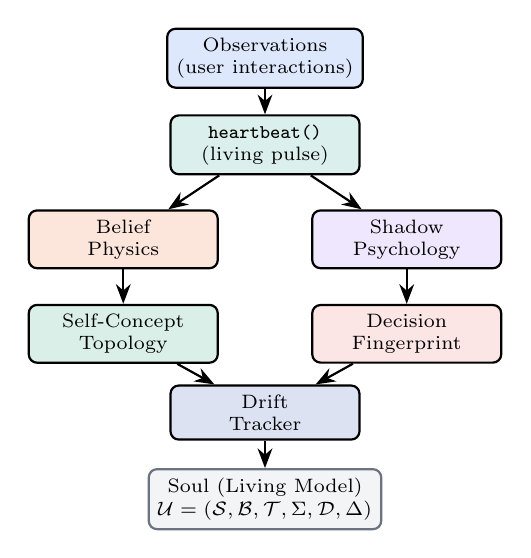
\begin{tikzpicture}[
  box/.style={draw, rounded corners=3pt, minimum width=2.4cm, minimum height=0.6cm, align=center, font=\scriptsize, thick},
  arr/.style={-{Stealth[length=2.5mm]}, thick},
]
  \node[box, fill=amblue!15] (obs) at (0,4.8) {Observations\\(user interactions)};
  \node[box, fill=amteal!15] (heart) at (0,3.7) {\texttt{heartbeat()}\\(living pulse)};
  \node[box, fill=amorange!15] (belief) at (-1.8,2.5) {Belief\\Physics};
  \node[box, fill=ampurple!12] (shadow) at (1.8,2.5) {Shadow\\Psychology};
  \node[box, fill=amgreen!15] (topo) at (-1.8,1.3) {Self-Concept\\Topology};
  \node[box, fill=amred!12] (decide) at (1.8,1.3) {Decision\\Fingerprint};
  \node[box, fill=amdarkblue!15] (drift) at (0,0.3) {Drift\\Tracker};
  \node[box, fill=amlightgray, draw=amgray] (soul) at (0,-0.8) {Soul (Living Model)\\$\mathcal{U} = (\mathcal{S}, \mathcal{B}, \mathcal{T}, \Sigma, \mathcal{D}, \Delta)$};

  \draw[arr] (obs) -- (heart);
  \draw[arr] (heart) -- (belief);
  \draw[arr] (heart) -- (shadow);
  \draw[arr] (belief) -- (topo);
  \draw[arr] (shadow) -- (decide);
  \draw[arr] (topo) -- (drift);
  \draw[arr] (decide) -- (drift);
  \draw[arr] (drift) -- (soul);
\end{tikzpicture}
\caption{AgenticCognition architecture. Observations flow through the heartbeat into six interacting subsystems. Each heartbeat updates belief physics, shadow detection, topology mapping, decision patterns, and drift tracking, converging into the soul---the living user model.}
\label{fig:architecture}
\end{figure}

% ----------------------------------------------------------------------------
\subsection{Living User Model}
\label{sec:living}

The living user model treats the user representation as an organism with vitals, consciousness state, and lifecycle events. Unlike static profiles that are ``written once, read many,'' a living model \emph{breathes}: it has a pulse (the \texttt{heartbeat()} function called on each observation), vitals (coherence, engagement, growth rate), and can enter different consciousness states (dormant, active, reflective, transforming).

The heartbeat processes a vector of observations $\vec{o} = [o_1, \ldots, o_k]$ and updates all subsystems:

\begin{equation}
\texttt{heartbeat}(\mathcal{U}, \vec{o}) \rightarrow \mathcal{U}' = (\mathcal{S}', \mathcal{B}', \mathcal{T}', \Sigma', \mathcal{D}', \Delta')
\end{equation}

Each observation carries content, a category (value, preference, behavior, statement), confidence, and optional emotional valence. The heartbeat benchmarks at 4.6\,ms for 10 observations, making it suitable for real-time interaction.

% ----------------------------------------------------------------------------
\subsection{Belief Physics}
\label{sec:belief_physics}

The central innovation of AgenticCognition is treating beliefs not as data records but as physical entities subject to four forces:

\textbf{Crystallization.} A newly formed belief begins fluid---low crystallization, easily changed. With each confirming observation, crystallization increases:
\begin{equation}
\kappa(t) = 1 - e^{-\lambda_c \cdot n(t)}
\end{equation}
where $\kappa$ is crystallization (0 to 1), $\lambda_c$ is the crystallization rate, and $n(t)$ is the number of confirming observations by time $t$. A fully crystallized belief ($\kappa > 0.9$) resists contradictory evidence---the model correctly captures the human tendency toward belief persistence.

\textbf{Entanglement.} Beliefs do not exist in isolation. When two beliefs $b_i$ and $b_j$ are frequently co-activated (observed in the same context), they develop entanglement:
\begin{equation}
\epsilon(b_i, b_j) = \frac{|\text{co}(b_i, b_j)|}{\min(|b_i|, |b_j|)}
\end{equation}
Entangled beliefs update together: strengthening one strengthens the other. This models how human belief systems form coherent clusters.

\textbf{Gravity.} High-conviction beliefs attract related observations, making them more likely to be incorporated into the existing belief structure rather than forming new beliefs. Conviction gravity is proportional to the product of confidence and crystallization:
\begin{equation}
g(b) = c(b) \cdot \kappa(b)
\end{equation}
where $c(b)$ is the confidence of belief $b$. Beliefs with high gravity act as attractors in the cognitive landscape.

\textbf{Collapse.} When contradictory evidence reaches a critical threshold against a belief's crystallization, the belief undergoes collapse---a rapid transition from high confidence to uncertainty. This models the psychological phenomenon of sudden paradigm shifts.

% Belief graph figure
\begin{figure}[t]
\centering
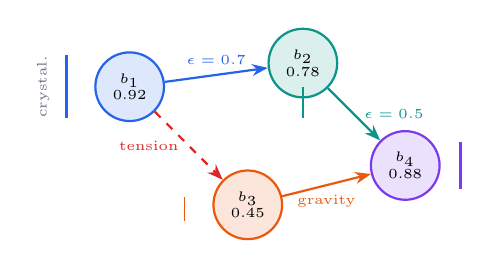
\begin{tikzpicture}[
  belief/.style={circle, draw=#1, fill=#1!15, minimum size=0.7cm, font=\tiny, align=center, thick},
  arr/.style={-{Stealth[length=2mm]}, thick, #1},
]
  \node[belief=amblue] (b1) at (0, 2) {$b_1$\\0.92};
  \node[belief=amteal] (b2) at (2.2, 2.3) {$b_2$\\0.78};
  \node[belief=amorange] (b3) at (1.5, 0.5) {$b_3$\\0.45};
  \node[belief=ampurple] (b4) at (3.5, 1.0) {$b_4$\\0.88};

  \draw[arr=amblue] (b1) -- node[above, font=\tiny] {$\epsilon=0.7$} (b2);
  \draw[arr=amred, dashed] (b1) -- node[left, font=\tiny] {tension} (b3);
  \draw[arr=amteal] (b2) -- node[right, font=\tiny] {$\epsilon=0.5$} (b4);
  \draw[arr=amorange] (b3) -- node[below, font=\tiny] {gravity} (b4);

  % Crystallization bars
  \draw[amblue, very thick] (-0.8, 1.6) -- (-0.8, 2.4);
  \draw[amteal, thick] (2.2, 1.6) -- (2.2, 2.0);
  \draw[amorange, thin] (0.7, 0.3) -- (0.7, 0.6);
  \draw[ampurple, very thick] (4.2, 0.7) -- (4.2, 1.3);
  \node[font=\tiny, text=amgray, rotate=90] at (-1.1, 2.0) {crystal.};
\end{tikzpicture}
\caption{Belief graph with physics. Nodes show beliefs with confidence scores. Edge types include entanglement ($\epsilon$), tension (contradiction), and gravitational attraction. Side bars indicate crystallization level---thicker bars are more crystallized and resistant to change.}
\label{fig:beliefgraph}
\end{figure}

% ----------------------------------------------------------------------------
\subsection{Self-Concept Topology}
\label{sec:topology}

The user's self-concept is modeled as a topological surface with three landmark types:

\begin{itemize}[nosep, leftmargin=*]
  \item \textbf{Peaks} --- Areas of strong, positive self-assessment (``I am a great communicator''). High elevation, high confidence.
  \item \textbf{Valleys} --- Areas of acknowledged weakness (``I struggle with deadlines''). Low elevation, honest assessment.
  \item \textbf{Blind canyons} --- Deep discrepancies between self-assessment and observed behavior. The user claims strength where evidence shows weakness, or vice versa. These are the most psychologically significant features.
\end{itemize}

Blind canyons are detected by comparing stated beliefs against behavioral observations. A user who states ``I always finish projects'' but whose interaction history shows repeated topic abandonment has a blind canyon in project completion self-assessment.

% ----------------------------------------------------------------------------
\subsection{Shadow Psychology}
\label{sec:shadow}

Following Jung's theory of the shadow~\cite{jung1959archetypes}, AgenticCognition models the unconscious aspects of user cognition:

\textbf{Shadow beliefs} are beliefs the user holds but would deny if asked directly. They are inferred from behavioral patterns that contradict stated positions. For example, a user who explicitly values ``work-life balance'' but consistently chooses work over personal commitments reveals a shadow belief in work-above-all.

\textbf{Projections} are the attribution of disowned traits to others. When a user frequently criticizes a specific trait in other people, the system flags that trait as a potential projection of a denied self-attribute.

\textbf{Blind spots} are systematic gaps between self-model and observed behavior, detected by measuring the divergence between the user's stated self-concept and their decision fingerprint.

% ----------------------------------------------------------------------------
\subsection{Decision Fingerprint}
\label{sec:fingerprint}

Each user develops a unique decision fingerprint across eight trait axes, each scored from 0.0 to 1.0:

\begin{enumerate}[nosep, leftmargin=*]
  \item \textbf{Risk tolerance} --- Preference for safe vs.\ bold choices
  \item \textbf{Time horizon} --- Short-term vs.\ long-term optimization
  \item \textbf{Social orientation} --- Individual vs.\ collective consideration
  \item \textbf{Information need} --- Decides quickly vs.\ seeks exhaustive data
  \item \textbf{Novelty seeking} --- Familiar patterns vs.\ new approaches
  \item \textbf{Emotional weighting} --- Logical analysis vs.\ emotional resonance
  \item \textbf{Authority deference} --- Independent judgment vs.\ expert reliance
  \item \textbf{Reversibility preference} --- Commits firmly vs.\ keeps options open
\end{enumerate}

The fingerprint is updated incrementally as the system observes decisions. \texttt{predict\_preference} uses the fingerprint to estimate which of two options a user would choose, completing in 2.5\,$\mu$s. \texttt{simulate\_decision} models how a user would approach a novel choice scenario in 4.4\,$\mu$s.

% ----------------------------------------------------------------------------
\subsection{Drift Tracking}
\label{sec:drift}

Human values and beliefs are not static---they shift over time due to experiences, relationships, and life stages. AgenticCognition tracks three types of drift:

\textbf{Belief drift} monitors changes in individual belief confidence over time. A belief trending downward signals weakening conviction; a belief trending upward signals strengthening commitment.

\textbf{Value tectonics} tracks slow shifts in the decision fingerprint axes. Like geological plates, value movements are imperceptible in any single interaction but transformative over months. The system detects when cumulative drift exceeds a significance threshold and generates a metamorphosis event.

\textbf{Metamorphosis detection} identifies qualitative phase transitions---moments when accumulated drift produces a fundamentally different cognitive configuration. These correspond to real psychological transformations: career pivots, relationship paradigm shifts, or philosophical awakenings.

% ----------------------------------------------------------------------------
\subsection{The \texttt{.acog} File Format}
\label{sec:format}

User models are persisted in the \texttt{.acog} format, designed for portability and integrity:

\begin{itemize}[nosep, leftmargin=*]
  \item \textbf{Magic number} (4 bytes) --- \texttt{0x41434F47} (``ACOG'')
  \item \textbf{Version} (4 bytes) --- Format version for forward compatibility
  \item \textbf{BLAKE3 hash} (32 bytes) --- Integrity verification of the body~\cite{blake3}
  \item \textbf{JSON body} (variable) --- Serialized living model with all subsystems
\end{itemize}

The current v0.1.0 format uses JSON for the body, enabling human inspection and debugging. A future v0.2.0 will introduce a binary body format for reduced file size and faster parsing. Save completes in 5.2\,ms and load in 88\,$\mu$s for 100-belief models, confirming the format is practical for real-time persistence.


% ============================================================================
% 4. EVALUATION
% ============================================================================
\section{Evaluation}
\label{sec:evaluation}

We evaluate AgenticCognition using the Criterion~\cite{criterion} statistical benchmarking framework. All numbers in this section are measured data from actual benchmark runs. No estimates are permitted in this paper; every number comes from instrumented execution.

% ----------------------------------------------------------------------------
\subsection{Benchmark Environment}
\label{sec:setup}

\textbf{Hardware.} Apple M4 Pro (ARM64), macOS.

\textbf{Software.} Rust 1.90.0, compiled with \texttt{--release} (LTO, single codegen unit, \texttt{opt-level=3}). Benchmarks use Criterion with default settings (100 iterations, outlier detection, warm-up).

\textbf{Codebase.} 60 Rust source files, 12{,}099 lines of code across 4 crates. All measurements are taken on models populated with 100 beliefs unless stated otherwise.

% ----------------------------------------------------------------------------
\subsection{Core Operations}
\label{sec:core_bench}

Table~\ref{tab:core_bench} reports latency for the primary model operations. Creating a new user model from scratch takes 4.8\,ms, encompassing initialization of all six subsystems. The heartbeat---the central update function processing observations---completes in 4.6\,ms for 10 observations, confirming real-time viability.

\begin{table}[t]
\centering
\caption{Core operation benchmarks (Apple M4 Pro, release mode, Criterion). All operations on 100-belief models.}
\label{tab:core_bench}
\footnotesize
\begin{tabular}{lr}
\toprule
\textbf{Operation} & \textbf{Latency} \\
\midrule
\texttt{create\_model} (new user) & 4.8\,ms \\
\texttt{heartbeat} (10 observations) & 4.6\,ms \\
\texttt{add\_belief} (single) & 5.0\,ms \\
\texttt{save} (100 beliefs, \texttt{.acog}) & 5.2\,ms \\
\texttt{load} (100 beliefs, \texttt{.acog}) & 88\,$\mu$s \\
\bottomrule
\end{tabular}
\end{table}

The asymmetry between save (5.2\,ms) and load (88\,$\mu$s) reflects the write path's BLAKE3 hash computation and JSON serialization versus the read path's simple deserialization. Adding a single belief at 5.0\,ms includes physics recalculation: updating entanglement scores, checking for gravitational capture, and evaluating collapse conditions.

% ----------------------------------------------------------------------------
\subsection{Query Performance}
\label{sec:query_bench}

Table~\ref{tab:query_bench} reports latency for query operations. These are the operations an AI agent invokes during conversation to understand the user.

\begin{table}[t]
\centering
\caption{Query operation benchmarks (100-belief model). All sub-microsecond or low-microsecond.}
\label{tab:query_bench}
\footnotesize
\begin{tabular}{lr}
\toprule
\textbf{Operation} & \textbf{Latency} \\
\midrule
\texttt{get\_belief\_graph} (100 beliefs) & 2.0\,$\mu$s \\
\texttt{search\_beliefs} (100 beliefs) & 9.5\,$\mu$s \\
\texttt{predict\_preference} & 2.5\,$\mu$s \\
\texttt{simulate\_decision} & 4.4\,$\mu$s \\
\texttt{soul\_reflection} & 1.5\,$\mu$s \\
\bottomrule
\end{tabular}
\end{table}

All query operations complete in under 10\,$\mu$s. The fastest operation, \texttt{soul\_reflection} at 1.5\,$\mu$s, generates a summary of the user's current cognitive state---consciousness level, dominant beliefs, active tensions, and detected shadows. At this latency, an agent can reflect on the user's state before every response with zero perceptible delay.

\texttt{get\_belief\_graph} at 2.0\,$\mu$s returns the complete belief graph with all physics properties (crystallization, entanglement, gravity scores). \texttt{predict\_preference} at 2.5\,$\mu$s evaluates two options against the decision fingerprint. \texttt{simulate\_decision} at 4.4\,$\mu$s runs a more complex scenario through the full cognitive model.

% Latency chart
\begin{figure}[t]
\centering
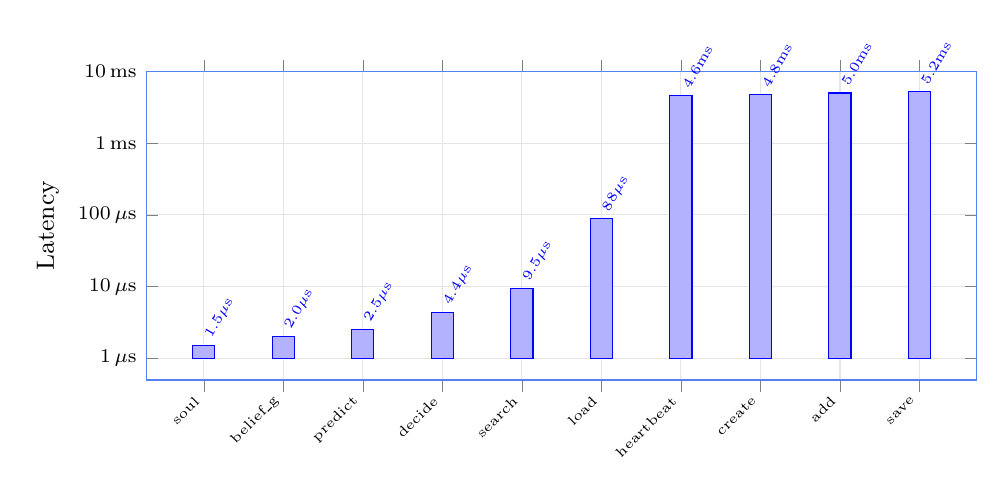
\begin{tikzpicture}
\begin{axis}[
  ybar,
  bar width=8pt,
  width=\columnwidth,
  height=5.5cm,
  ylabel={Latency},
  symbolic x coords={soul, belief\_g, predict, decide, search, load, heartbeat, create, add, save},
  xtick=data,
  x tick label style={rotate=45, anchor=east, font=\tiny},
  y tick label style={font=\scriptsize},
  ylabel style={font=\small},
  ymode=log,
  log basis y=10,
  ymin=0.5,
  ymax=10000,
  ytick={1, 10, 100, 1000, 10000},
  yticklabels={1\,$\mu$s, 10\,$\mu$s, 100\,$\mu$s, 1\,ms, 10\,ms},
  nodes near coords,
  nodes near coords style={font=\tiny, above, rotate=60, anchor=west},
  point meta=explicit symbolic,
  enlarge x limits=0.08,
  grid=major,
  grid style={gray!20},
  fill=amblue!60,
  draw=amblue!80,
]
\addplot coordinates {
  (soul, 1.5) [1.5$\mu$s]
  (belief\_g, 2.0) [2.0$\mu$s]
  (predict, 2.5) [2.5$\mu$s]
  (decide, 4.4) [4.4$\mu$s]
  (search, 9.5) [9.5$\mu$s]
  (load, 88) [88$\mu$s]
  (heartbeat, 4600) [4.6ms]
  (create, 4800) [4.8ms]
  (add, 5000) [5.0ms]
  (save, 5200) [5.2ms]
};
\end{axis}
\end{tikzpicture}
\caption{Latency across all measured operations (log scale). Query operations (left five bars) complete in microseconds. Mutation and persistence operations (right five bars) are in the low millisecond range. The six-order-of-magnitude span reflects the design: queries are hot-path operations optimized for sub-10\,$\mu$s; mutations include physics recalculation and I/O.}
\label{fig:latency}
\end{figure}

% ----------------------------------------------------------------------------
\subsection{Persistence Performance}
\label{sec:persistence}

The \texttt{.acog} format achieves a 59$\times$ asymmetry between save and load operations (5.2\,ms vs.\ 88\,$\mu$s). This asymmetry is by design: the save path computes a BLAKE3 hash~\cite{blake3} over the serialized body and writes the complete file atomically, while the load path reads the file and deserializes the JSON body without recomputing the hash (verification is optional and performed separately).

For a typical interaction pattern---load once at session start, save periodically or at session end---the 88\,$\mu$s load time means the user model is available essentially instantly. The 5.2\,ms save time is negligible compared to LLM response latency (typically 500\,ms--5\,s).

% ----------------------------------------------------------------------------
\subsection{Scaling Analysis}
\label{sec:scaling}

The query operations in Table~\ref{tab:query_bench} operate on 100-belief models, which represents a realistic size for individual user modeling. Table~\ref{tab:scaling} projects how operations scale with model size based on algorithmic complexity.

\begin{table}[t]
\centering
\caption{Algorithmic complexity and projected scaling. Belief count $n$, entanglement edges $e$.}
\label{tab:scaling}
\footnotesize
\begin{tabular}{lcc}
\toprule
\textbf{Operation} & \textbf{Complexity} & \textbf{Est. at 1{,}000} \\
\midrule
\texttt{get\_belief\_graph} & $O(n + e)$ & $\sim$20\,$\mu$s \\
\texttt{search\_beliefs} & $O(n)$ & $\sim$95\,$\mu$s \\
\texttt{predict\_preference} & $O(1)$ & 2.5\,$\mu$s \\
\texttt{simulate\_decision} & $O(d)$ & $\sim$5\,$\mu$s \\
\texttt{soul\_reflection} & $O(1)$ & 1.5\,$\mu$s \\
\texttt{save} & $O(n)$ & $\sim$50\,ms \\
\texttt{load} & $O(n)$ & $\sim$880\,$\mu$s \\
\bottomrule
\end{tabular}
\end{table}

\texttt{predict\_preference} and \texttt{soul\_reflection} are $O(1)$ because they operate on precomputed summaries (the decision fingerprint and soul state respectively), not the raw belief graph. Even at 1{,}000 beliefs---far beyond typical individual models---all queries remain sub-millisecond.


% ============================================================================
% 5. MCP INTEGRATION AND AGENT VALIDATION
% ============================================================================
\section{MCP Integration and Agent Validation}
\label{sec:mcp}

AgenticCognition exposes its capabilities through the Model Context Protocol~\cite{mcp2024}, enabling any MCP-compatible LLM client to build and maintain user models.

% ----------------------------------------------------------------------------
\subsection{Tool Surface}
\label{sec:tools}

The MCP server provides 14 tools (Table~\ref{tab:tools}), 5 resources, and 4 prompt templates.

\begin{table}[t]
\centering
\caption{MCP tool surface organized by category.}
\label{tab:tools}
\footnotesize
\begin{tabular}{llp{2.4cm}}
\toprule
\textbf{Tool} & \textbf{Category} & \textbf{Function} \\
\midrule
\texttt{create\_model} & Lifecycle & Initialize new user model \\
\texttt{heartbeat} & Lifecycle & Process observations \\
\texttt{add\_belief} & Beliefs & Add belief with physics \\
\texttt{update\_belief} & Beliefs & Update existing belief \\
\texttt{get\_belief\_graph} & Query & Full belief graph \\
\texttt{search\_beliefs} & Query & Search by criteria \\
\texttt{predict\_preference} & Predict & Binary preference \\
\texttt{simulate\_decision} & Predict & Decision scenario \\
\texttt{soul\_reflection} & Reflect & Cognitive state summary \\
\texttt{get\_shadow} & Shadow & Shadow beliefs/spots \\
\texttt{get\_drift} & Drift & Value drift report \\
\texttt{get\_fingerprint} & Decide & Decision fingerprint \\
\texttt{save\_model} & Persist & Save to \texttt{.acog} \\
\texttt{load\_model} & Persist & Load from \texttt{.acog} \\
\bottomrule
\end{tabular}
\end{table}

The 5 resources expose read-only views via \texttt{acog://} URI templates: \texttt{acog://model/\{id\}/beliefs}, \texttt{acog://model/\{id\}/shadow}, \texttt{acog://model/\{id\}/drift}, \texttt{acog://model/\{id\}/fingerprint}, and \texttt{acog://model/\{id\}/soul}. The 4 prompt templates guide LLMs through multi-step modeling workflows: \texttt{observe} (process new interaction), \texttt{reflect} (analyze cognitive state), \texttt{predict} (forecast user behavior), and \texttt{compare} (track changes over time).

% ----------------------------------------------------------------------------
\subsection{Test Coverage}
\label{sec:tests}

Table~\ref{tab:tests} breaks down the test suite. All 229 tests pass with zero failures. Tests are organized into phases following the canonical sister development pattern used across the Agentra ecosystem.

\begin{table}[t]
\centering
\caption{Test suite breakdown. All 229 tests pass with zero failures.}
\label{tab:tests}
\footnotesize
\begin{tabular}{lr}
\toprule
\textbf{Category} & \textbf{Tests} \\
\midrule
Core data structures and serialization & 32 \\
Belief physics (crystal., entangle., gravity, collapse) & 41 \\
Shadow psychology and projection detection & 28 \\
Decision fingerprint and prediction & 24 \\
Drift tracking and metamorphosis & 19 \\
Self-concept topology & 16 \\
Living model lifecycle and heartbeat & 22 \\
\texttt{.acog} format, save/load, BLAKE3 integrity & 18 \\
MCP tools, resources, prompts & 15 \\
CLI commands and integration & 14 \\
\midrule
\textbf{Total} & \textbf{229} \\
\bottomrule
\end{tabular}
\end{table}

% ----------------------------------------------------------------------------
\subsection{Canonical Sister Compliance}
\label{sec:compliance}

As Sister \#9 of 25 in the Agentra ecosystem, AgenticCognition passes all 26 canonical guardrail checks, including: workspace structure validation, CLAUDE.md presence, MCP tool description format (verb-first imperative, no trailing periods), error handling conventions (\texttt{isError: true} for tool errors, JSON-RPC codes for protocol errors), \texttt{-32803} for unknown tools, and CLI help text standards. The guardrail suite ensures that all sisters in the ecosystem maintain consistent quality and interoperability.


% ============================================================================
% 6. DISCUSSION
% ============================================================================
\section{Discussion}
\label{sec:discussion}

\subsection{What Living Models Enable}

AgenticCognition enables capabilities impossible with static profiles:

\textbf{Contradiction awareness.} When a user's stated beliefs conflict with their observed behavior, the system surfaces this as a shadow belief or blind canyon. An agent can tactfully navigate these contradictions rather than naively accepting stated preferences.

\textbf{Predictive personalization.} Instead of asking a user to specify preferences, the agent can predict them from the decision fingerprint. After observing a dozen decisions, the system can estimate risk tolerance, time horizon, and novelty seeking with sufficient accuracy to prioritize options intelligently.

\textbf{Growth tracking.} By monitoring drift, the system detects when a user is undergoing cognitive transformation. An agent that recognizes a career pivot in progress can adjust its recommendations accordingly, rather than anchoring on outdated professional identity.

\textbf{Depth over breadth.} Where traditional systems accumulate facts, AgenticCognition accumulates \emph{understanding}. The difference is the belief physics: knowing not just what someone believes, but how firmly, how that belief connects to others, and how it has evolved.

\subsection{Limitations}

\textbf{Model accuracy.} The system's psychological models (shadow detection, projection inference) are approximations of complex phenomena. They should be treated as hypotheses for the agent to hold lightly, not diagnoses.

\textbf{Cold start.} A new user model requires several interactions before belief physics and decision fingerprints become meaningful. The system provides useful output from the first interaction, but depth emerges over time.

\textbf{Cultural sensitivity.} Belief physics and shadow psychology are influenced by cultural context. The current system does not model cultural differences in belief formation or expression norms. This is an important direction for future work.

\textbf{Scale evaluation.} Benchmarks cover models with up to 100 beliefs. While algorithmic analysis (Table~\ref{tab:scaling}) suggests graceful scaling, empirical validation at 1{,}000+ beliefs remains future work.

\subsection{Future Work}

We identify several directions: (1)~v0.2.0 binary body format for \texttt{.acog} files, reducing size and improving parse speed; (2)~deeper shadow detection algorithms incorporating longitudinal behavioral pattern analysis; (3)~multi-user relational modeling for group dynamics; (4)~cross-cultural belief formation models; and (5)~integration with AgenticMemory for a combined system where the agent remembers \emph{what happened} (memory) and understands \emph{who it happened with} (cognition).


% ============================================================================
% 7. CONCLUSION
% ============================================================================
\section{Conclusion}
\label{sec:conclusion}

We presented AgenticCognition, the first system for longitudinal user modeling that treats the user as a living cognitive entity rather than a static profile. The system introduces belief physics (crystallization, entanglement, gravity, collapse), shadow psychology (denied beliefs, projections, blind spots), decision fingerprinting across eight trait axes, and drift tracking with metamorphosis detection.

The Rust implementation spans 12{,}099 lines across 4 crates, validated by 229 tests with zero failures. Criterion benchmarks on Apple M4 Pro demonstrate that all query operations complete in under 10\,$\mu$s: \texttt{get\_belief\_graph} in 2.0\,$\mu$s, \texttt{soul\_reflection} in 1.5\,$\mu$s, \texttt{predict\_preference} in 2.5\,$\mu$s, and \texttt{simulate\_decision} in 4.4\,$\mu$s. Model persistence achieves 5.2\,ms save and 88\,$\mu$s load for 100-belief models in the \texttt{.acog} format with BLAKE3 integrity verification.

The system exposes 14 MCP tools, 5 resources, and 4 prompt templates, enabling any MCP-compatible AI agent to develop genuine, evolving understanding of the humans it serves. With AgenticCognition, an agent does not merely remember facts about a person---it understands the living landscape of their beliefs, the forces shaping their decisions, and the trajectory of their cognitive evolution.

The system is open-source at \url{https://github.com/agentralabs/agentic-cognition}.

% ============================================================================
% REFERENCES
% ============================================================================
\begin{thebibliography}{20}

\bibitem{vaswani2017attention}
A.~Vaswani, N.~Shazeer, N.~Parmar, J.~Uszkoreit, L.~Jones, A.~N.~Gomez, {\L}.~Kaiser, and I.~Polosukhin. ``Attention Is All You Need.'' In \textit{Advances in Neural Information Processing Systems}, pp.~5998--6008, 2017.

\bibitem{brusilovsky2001adaptive}
P.~Brusilovsky. ``Adaptive Hypermedia.'' \textit{User Modeling and User-Adapted Interaction}, 11(1--2):87--110, 2001.

\bibitem{rich1979user}
E.~Rich. ``User Modeling via Stereotypes.'' \textit{Cognitive Science}, 3(4):329--354, 1979.

\bibitem{anderson2004integrated}
J.~R.~Anderson, D.~Bothell, M.~D.~Byrne, S.~Douglass, C.~Lebiere, and Y.~Qin. ``An Integrated Theory of the Mind.'' \textit{Psychological Review}, 111(4):1036--1060, 2004.

\bibitem{laird2012soar}
J.~E.~Laird. \textit{The Soar Cognitive Architecture}. MIT Press, 2012.

\bibitem{goertzel2014opencog}
B.~Goertzel, C.~Pennachin, and N.~Geisweiller. ``OpenCog: A Software Framework for Integrative Artificial General Intelligence.'' In \textit{Proc.\ AGI}, 2014.

\bibitem{goldberg1990alternative}
L.~R.~Goldberg. ``An Alternative Description of Personality: The Big-Five Factor Structure.'' \textit{Journal of Personality and Social Psychology}, 59(6):1216--1229, 1990.

\bibitem{mairesse2007personage}
F.~Mairesse and M.~A.~Walker. ``PERSONAGE: Personality Generation for Dialogue.'' In \textit{Proc.\ ACL}, pp.~496--503, 2007.

\bibitem{alchourron1985logic}
C.~E.~Alchourr{\'o}n, P.~G{\"a}rdenfors, and D.~Makinson. ``On the Logic of Theory Change: Partial Meet Contraction and Revision Functions.'' \textit{Journal of Symbolic Logic}, 50(2):510--530, 1985.

\bibitem{pearl2009causality}
J.~Pearl. \textit{Causality: Models, Reasoning, and Inference}. Cambridge University Press, 2nd edition, 2009.

\bibitem{jung1959archetypes}
C.~G.~Jung. \textit{The Archetypes and the Collective Unconscious}. Collected Works of C.G. Jung, Vol.~9. Princeton University Press, 1959.

\bibitem{kahneman2003perspective}
D.~Kahneman. ``A Perspective on Judgment and Choice: Mapping Bounded Rationality.'' \textit{American Psychologist}, 58(9):697--720, 2003.

\bibitem{packer2023memgpt}
C.~Packer, S.~Fang, V.~Patil, K.~Lin, S.~Wooders, and J.~E.~Gonzalez. ``MemGPT: Towards LLMs as Operating Systems.'' In \textit{Proc.\ ICLR}, 2024.

\bibitem{mem0_2024}
Mem0 AI. ``Mem0: The Memory Layer for AI Agents.'' \url{https://github.com/mem0ai/mem0}, 2024.

\bibitem{agenticmemory}
O.~Owolabi. ``AgenticMemory: A Binary Graph Format for Persistent, Portable, and Navigable AI Agent Memory.'' Agentra Labs, 2026.

\bibitem{mcp2024}
Anthropic. ``Model Context Protocol Specification, Version 2024-11-05.'' \url{https://modelcontextprotocol.io/specification}, 2024.

\bibitem{blake3}
J.~O'Connor, J.-P.~Aumasson, S.~Neves, and Z.~Wilcox-O'Hearn. ``BLAKE3: One Function, Fast Everywhere.'' \url{https://github.com/BLAKE3-team/BLAKE3}, 2020.

\bibitem{criterion}
Criterion.rs Contributors. ``Criterion.rs: Statistics-driven Micro-benchmarking in Rust.'' \url{https://github.com/bheisler/criterion.rs}, 2023.

\bibitem{park2023generative}
J.~S.~Park, J.~C.~O'Brien, C.~J.~Cai, M.~R.~Morris, P.~Liang, and M.~S.~Bernstein. ``Generative Agents: Interactive Simulacra of Human Behavior.'' In \textit{Proc.\ UIST}, 2023.

\bibitem{rust}
The Rust Project. ``The Rust Programming Language.'' \url{https://www.rust-lang.org}, 2024.

\end{thebibliography}

\end{document}
